\chapter{Cloud Security}
La IT security è un insieme complesso di tecniche e tecnologie di regolamentazione riguardo due aspetti importanti: i regolamenti utilizzati per implementare le politiche di sicurezza all'interno di un'azienda, e i comportamenti che vengono utilizzati. Questo secondo aspetto è molto importante ed è stato possibile vederlo da vicino con l'app Immuni: è stata progettata con estrema cura da esperti del settore in sicurezza e privacy, ma non si è compresa la natura socio-tecnica dell'esperimento, a causa degli "strani" comportamenti del Bluetooth Low Energy, che fatica a comprendere quando dover registrare un contatto o meno, e a che distanza. Il fallimento di Immuni è dovuto al fatto che ci si è concentranti solo sulla parte tecnica dell'esperimento.

\vspace{5mm}

Lo scopo della security è proteggere l'integrita dei dati e l'accesso ad essi, sia da intenti maliziosi che da eventuali errori. Alcuni concetti base:
\begin{itemize}
    \item La \textbf{confidenzialità} implica che un messaggio scambiato tra provider e consumer non possa essere intercettato e visto da qualcuno non autorizzato.
    \item L'\textbf{integrità} consiste nell'evitare che il messaggio sia alterato da qualcuno non autorizzato. L'integrità non vale solo per la trasmissione ma anche per lo storage.
    \item L'\textbf{autenticazione} significa essere in grado di definire chi ha fornito questi dati, ovvero poter risalire ad una sorgente.
    \item La \textbf{non repudiation} indica poter provare che l'interazione effettuata è stata davvero effettuata.
    \item L'\textbf{availability} implica che una risorsa sia sempre disponibile per un periodo di tempo specifico. È una responsabilità condivisa tra cloud provider e cloud carrier, che di solito devono mantenere i log per un certo periodo di tempo stabilito dal SLA.
    \item Per \textbf{minaccia} (threat) si indica qualsiasi cosa che mette a rischio e può danneggiare le difese messe in atto dal sistema; possono essere manuali o costruite in maniera automatica per sfruttare le vulnerabilità note. Un attacco è definito come una minaccia che ottiene dei risultati.
    \item Una \textbf{vulnerabilità} è un qualsiasi tipo di debolezza che può essere dovuta a errori di configurazione, di policy, degli sviluppatori, o a causa di poche misure di sicurezza nell'architettura.
    \item Un \textbf{rischio} è la possibilità di subire perdite o danneggiamenti durante un'attività e viene misurata rispetto al livello della minaccia con delle metriche:
    \begin{itemize}
        \item probabilità di una minaccia di avvenire;
        \item attesa di danni dopo che la risorsa è stata compromessa.
    \end{itemize}
\end{itemize}
In generale tutti i controlli di sicurezza sono le contromisure adatte per controllare queste minacce, quindi vanno stabilite regole chiare e buone prassi che specificano come progettare e implementare un sistema per offrire il massimo della protezione.

\section{Threat agents}
Un threat agent è un'entità capace di effettuare un attacco, che può essere interno o esterno al cloud, umano o automatizzato. La figura illustra un ruolo che un threat agent assume in relazione alle vulnerabilità, alle minacce e ai rischi.

\begin{figure}[htb!]
    \centering
    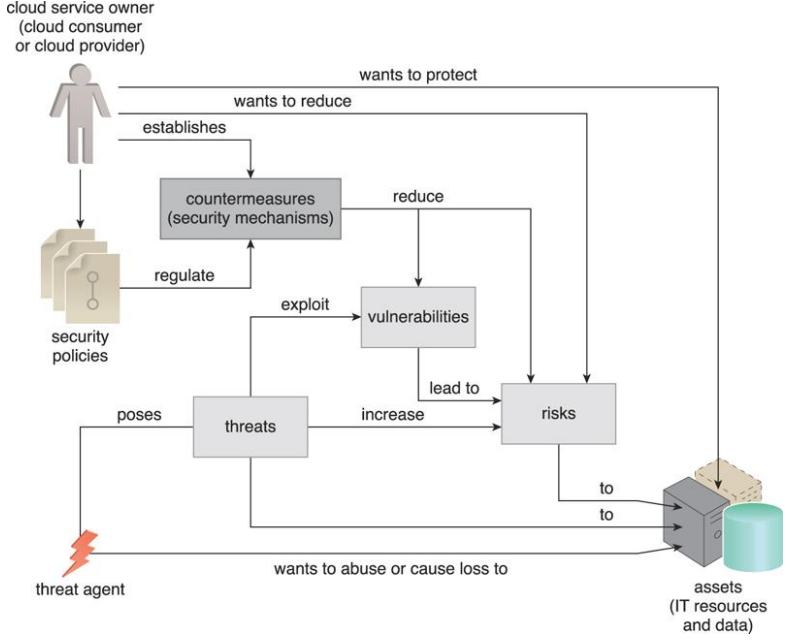
\includegraphics[width=9cm]{./Images/cap7/7.1.png}
\end{figure}

Le security policies sono stabilite dal cloud service owner e regolano le contromisure che hanno come obiettivo quello di fornire salvaguardia alle risorse. Distiguiamo diversi tipi di agenti:
\begin{itemize}
    \item \textbf{Anonymous attacker}: un agente esterno che consuma il servizio senza permessi, tipicamente è un programma che lancia attacchi a livello di network o ruba le credenziali di un utente.
    \item \textbf{Malicious service}: intercetta il traffico e può far credere di essere un service agent reale. Può essere anche un programma esterno che si occupa di intercettare i messaggi.
    \item \textbf{Trusted attacker}: è un attaccanteche condivide le risorse del provider con altri consumer e può attaccare i loro punti deboli, quindi più pericoloso degli altri perché già possiede parecchi permessi.
    \item \textbf{Malicious insider}: lavora dall'interno del cloud provider, quindi vanno controllati con cautela gli impiegati e la loro conoscenza di meccanismi o password che possono portare a terze parti non autorizzate ad avere accesso al sistema.
\end{itemize}
Le minacce che possono colpire il sistema sono:
\begin{itemize}
    \item \textbf{Traffic eavesdropping}: il traffico che viene trasferito da un cloud consumer ad un cloud provider e viceversa che viene intercettato da un agente esterno, può compromettere la confidenzialità dei dati, ed essendo un attacco passivo può essere notato anche dopo molto tempo.
    \item \textbf{Malicious intermediary}: un intermediario accede al messaggio e ne altera il contenuto, danneggiandone confidenzialità e integrità.
    \item \textbf{Denial of Service}: l'attacco più diffuso il cui obiettivo è quello di sovraccaricare le risorse del server in modo da comprometterne il corretto funzionamento. Può essere attuato aumentando artificialmente la mole di informazioni da scambiare e lavorando sulla rete occupando tutte le connessioni, oppure inviare richieste mirate che consumano le risorse disponibili.
    
    Il traffico che genera l'attaccante impedisce a richieste valide di poter essere fruite. Il problema di un DoS attack è che se il sistema scala automaticamente potrebbe causare costi molto elevati, soprattutto se l'attacco dura a lungo e non viene notato subito.
    \item \textbf{Insufficient authorization}: consiste nel non mettere in atto contromisure permettendo ad un attaccante di accedere a risorse IT che normalmente dovrebbero essere protette. Può essere risolto implementando l'autenticazione a due fattori.
    \item \textbf{Virtualization attack}: tipico della sicurezza del cloud, perché si basa sul concetto di una singola risorsa fisica che virtualizza più risorse logiche. Se una macchina logica viene attaccata con successo, potrebbe essere compromessa anche la macchina fisica e di conseguenza le altre macchine logiche in esecuzione su di essa.
    \item \textbf{Overlapping trust boundaries}: quando diversi consumer condividono delle risorse sul provider, un attacco ad uno di loro può compromettere anche l'altro.
\end{itemize}
I possibili problemi che vanno tenuti d'occhio riguardano le implementazioni di software con exploit, perché un errore che avviene in una certa implementazione può compromettere anche le altre.

\begin{figure}[htb!]
    \centering
    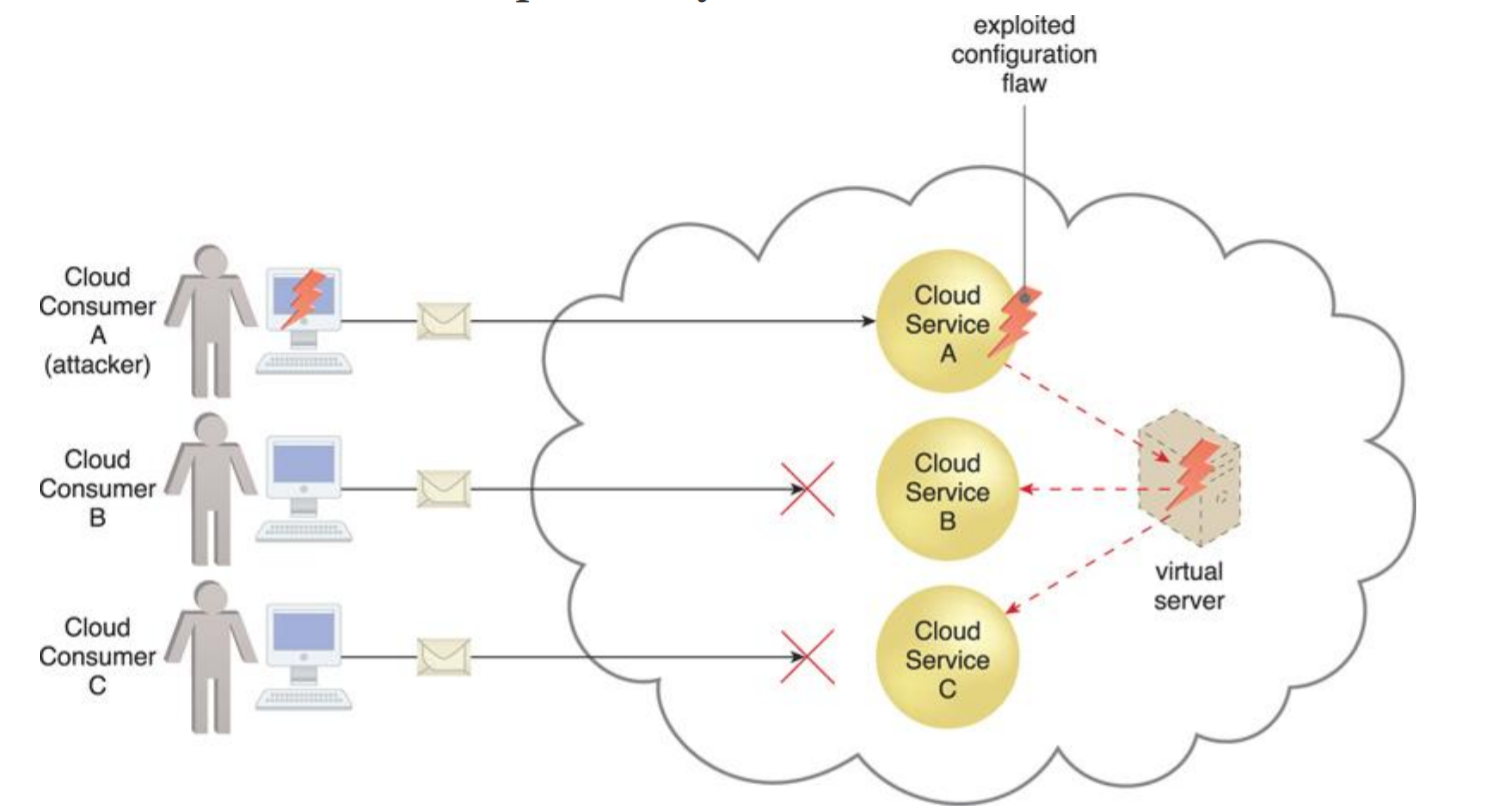
\includegraphics[width=7cm]{./Images/cap7/7.2.png}
\end{figure}

Ci sono poi problemi dovuti alle policy di sicurezza: bisogna considerare che non sempre consumer e provider attuano le stesse policy, e questo può accadere per diversi motivi, primo tra tutti il budget a disposizione per la IT security. Se ad esempio la sicurezza da parte del consumer è molto bassa, la sicurezza totale del sistema diminuisce in quanto il sistema è tanto forte quanto il suo anello più debole. Questo implica che la sicurezza non è un problema soltanto del provider, ed è per ciò che esistono gli \textit{assessment di incompatibilità}, ovvero limitazioni che spesso vengono messe in atto dal provider nei confronti del consumer (limitati aggiornamenti alla macchina in uso, permessi non di amministratore, ecc.).

Tutte le policy di sicurezza vengono specificate nel SLA assieme alle responsabilità che assume il cloud provider. Maggiore è la responsabilità del provider, minore è il rischio del consumer, ma maggiori saranno le restrizioni che il provider imporrà. 

\section{Risk Management}
Nei sistemi IT di grandi dimensioni il Risk Management va attuato nei data center. Negli ambienti cloud ci sono molteplici attori quindi il rischio va calcolato per ogni attore. Il compito del provider è quello di partizionare le risorse in modo che il risk management sia fatto in rapporto 1:1 con i vari consumer, mentre il compito dei consumer è essere sicuro che il risk management fatto dal provider sia adeguato ai costi richiesti. 

Il Risk Management è un processo ciclico che deve essere ripetuto per assicurare sicurezza strategica (a livello di sistema) e tattica (a livello di componenti), e può essere iniziato da qualsiasi fase. Di seguito sono illustrate le diverse fasi.

\subsubsection{\textbf{ASSESSMENT}}
Nella prima fase vanno identificate le potenziali vulnerabilità, visualizzando le statistiche a disposizione e estraendone le informazioni utili per la quantificazione del rischio, sulla base della probabilità di occorrenza di certe situazioni.

\begin{figure}[htb!]
    \centering
    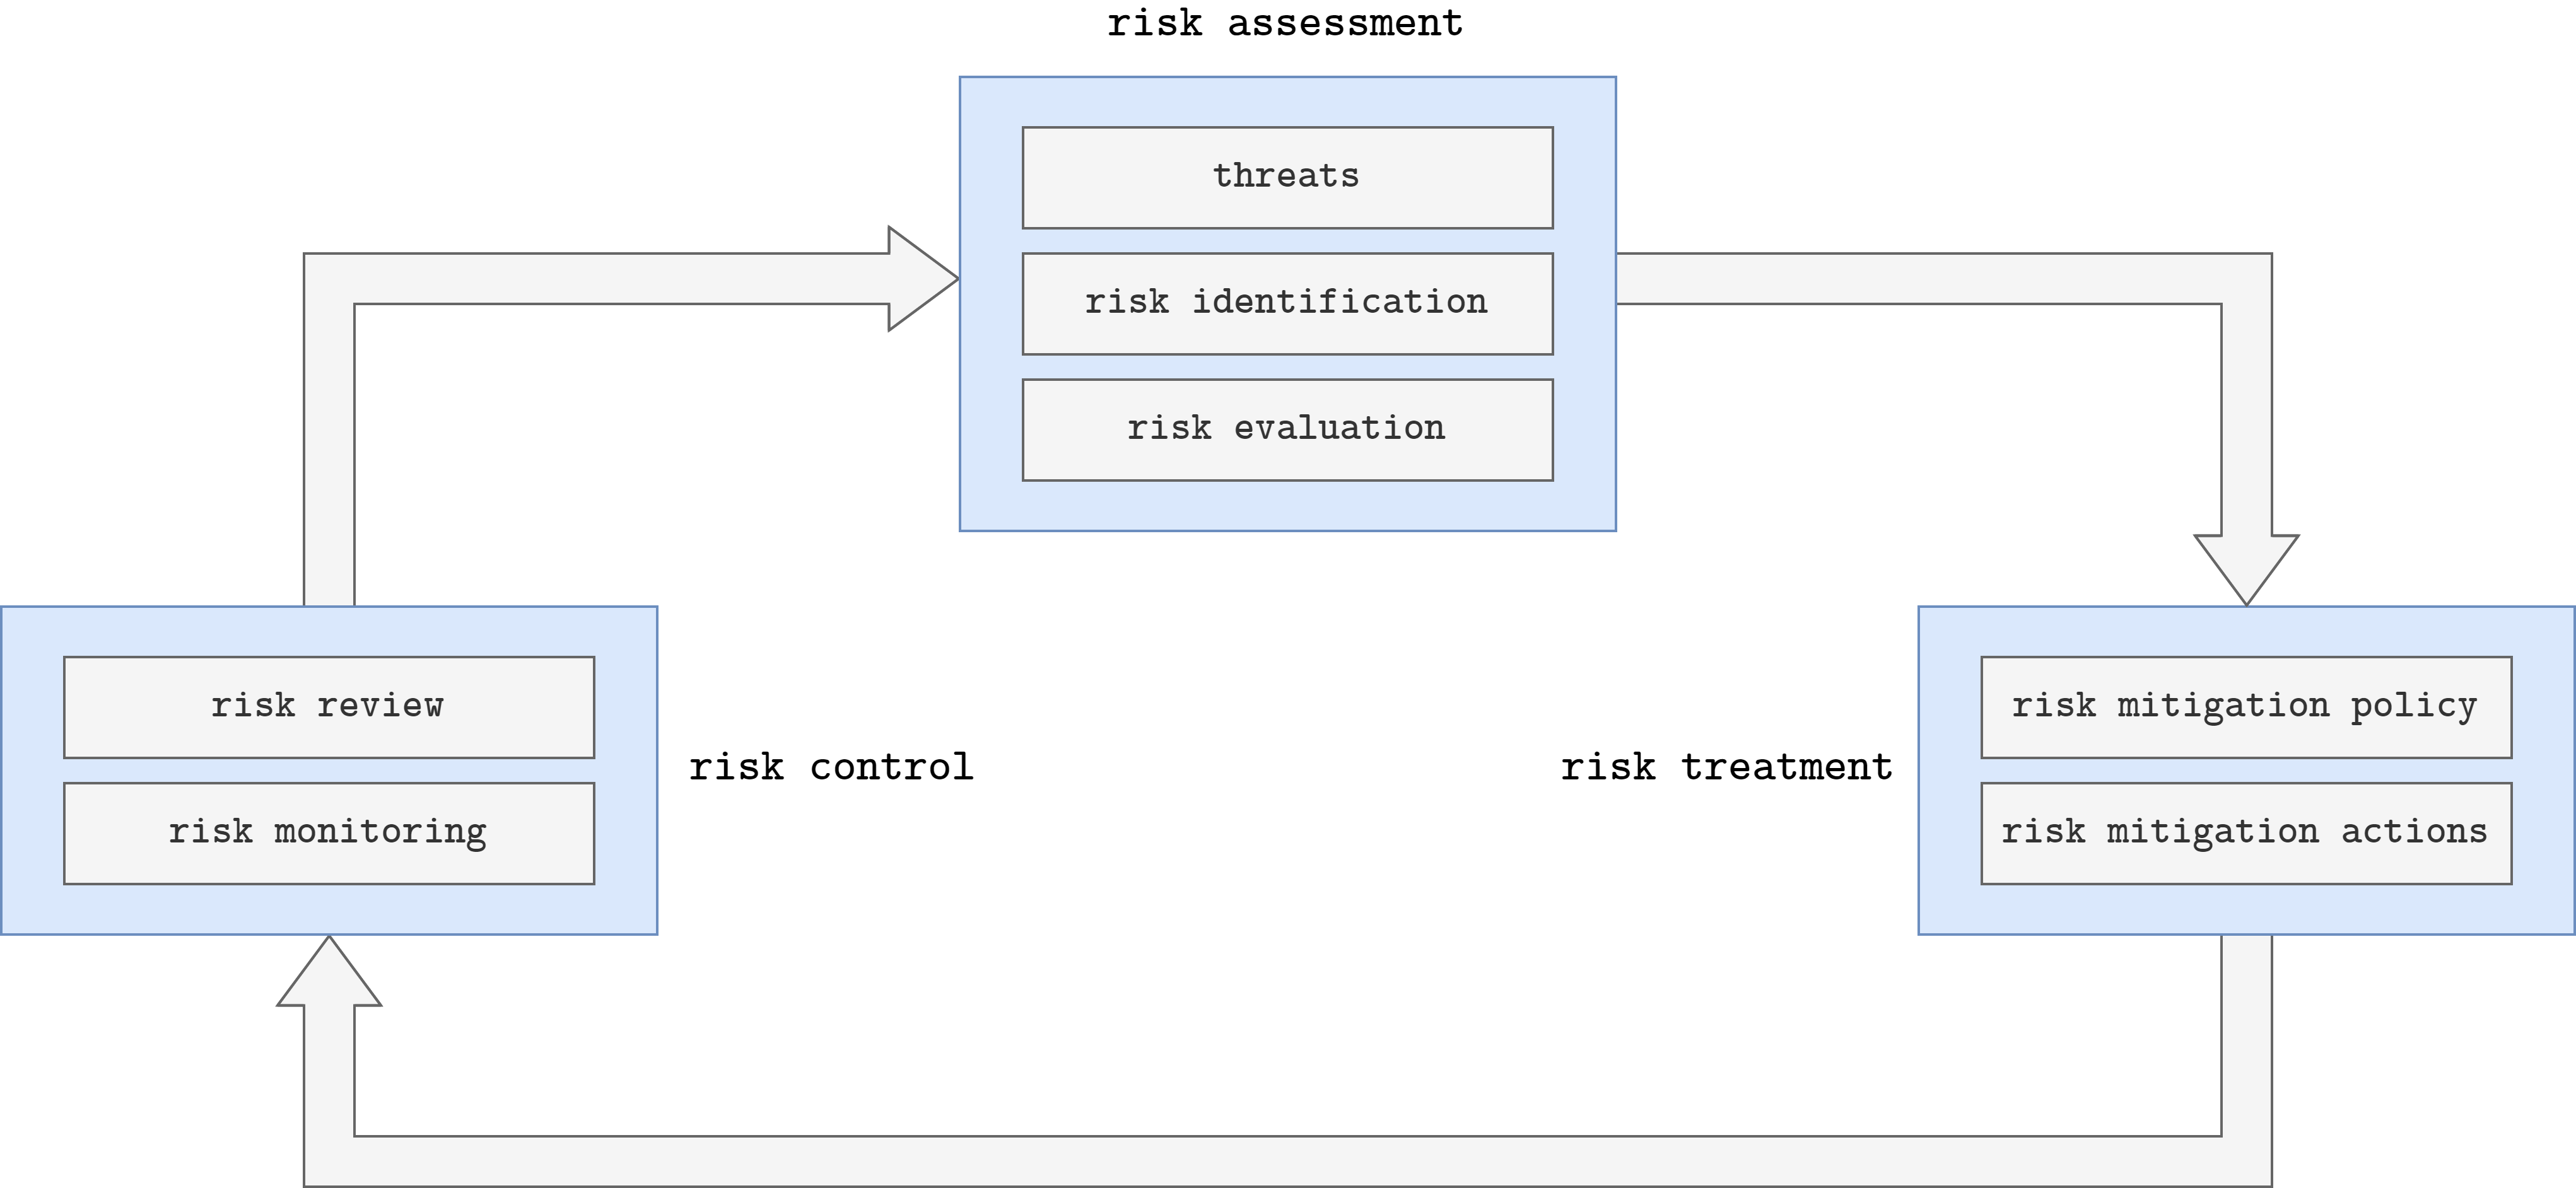
\includegraphics[width=9cm]{./Images/cap7/7.3.png}
\end{figure}

\subsubsection{\textbf{TREATMENT}}
Una volta scoperti i rischi, bisogna cercare di definire delle politiche per arginarli e cosa fare nel caso si verifichino. Alcuni rischi possono essere eliminati, altri solo mitigati, per altri è possibile rivolgersi a terze parti oppure in certi casi si è disposti a perdere una parte del budget. La parte di risk treatment viene affrontata nei SLA.

\subsubsection{\textbf{CONTROL}}
Il risk control avviene dopo. Come dice il saggio, \textit{"shit happens"}, quindi bisogna monitorare le soluzioni attuate e capire se hanno risolto o meno il problema. Alla fine di questa fase, viene effettuato di nuovo un assessment per stabilire quali sono le nuove vulnerabilità e quali sono state risolte.
\clearpage

\subsection{Risk Management Framework}
La tabella mostra le fasi di un corretto risk management e gli step che le compongono.

% \usepackage{multirow}
% \usepackage{colortbl}


\begin{table}[htb!]
\centering
\begin{tabular}{|c|l|} 
\hline
\rowcolor[rgb]{0.902,0.902,0.902} \textbf{CRMF}                           & \multicolumn{1}{c|}{\textbf{CRMF Steps}}                                                                                                                                                                                                                         \\ 
\hline
\multirow{2}{*}{\begin{tabular}[c]{@{}c@{}}Risk\\assessment\end{tabular}} & \begin{tabular}[c]{@{}l@{}}\textbf{Step 1. }Si categorizza il sistema e tutto quello che processa,\\in breve calcolo e storage.\end{tabular}                                                                                                                     \\ 
\cline{2-2}
                                                                          & \begin{tabular}[c]{@{}l@{}}\textbf{Step 2. }Si itentificano una serie di controlli di sicurezza in modo \\che siano proporzionali al rischio e si sviluppa una strategia per \\il monitoring.\end{tabular}                                                       \\ 
\hline
\multirow{2}{*}{\begin{tabular}[c]{@{}c@{}}Risk\\Treatment\end{tabular}}  & \begin{tabular}[c]{@{}l@{}}\textbf{Step 3. }Bisogna interpretare i security control e descrivere come \\tutti i controlli arrivano al security plan e come vengono portati \\all'interno del sistema.\end{tabular}                                               \\ 
\cline{2-2}
                                                                          & \begin{tabular}[c]{@{}l@{}}\textbf{Step 4. }Si verificano i security control con le procedure di risk \\assessment. Sono fasi importanti perché non coinvolgono le \\stesse persone.\end{tabular}                                                                \\ 
\hline
\multirow{2}{*}{\begin{tabular}[c]{@{}c@{}}Risk\\control\end{tabular}}    & \begin{tabular}[c]{@{}l@{}}\textbf{Step 5. }Si valuta se il rischio è accettabile in quanto dipende \\direttamente dalla \textit{mission }dell'azienda. Non bisogna dimenticare \\che il rischio agisce sul nome e sulla reputazione dell'azienda.\end{tabular}  \\ 
\cline{2-2}
                                                                          & \begin{tabular}[c]{@{}l@{}}\textbf{Step 6. }Si monitorano i controlli di sicurezza per dare feedback \\necessari alle fasi successive del ciclo.\end{tabular}                                                                                                    \\
\hline
\end{tabular}
\end{table}

Il grafico seguente invece mostra come sono divise le responsabilità nei vari deployment models tra cloud consumer e cloud provider.

\begin{figure}[htb!]
    \centering
    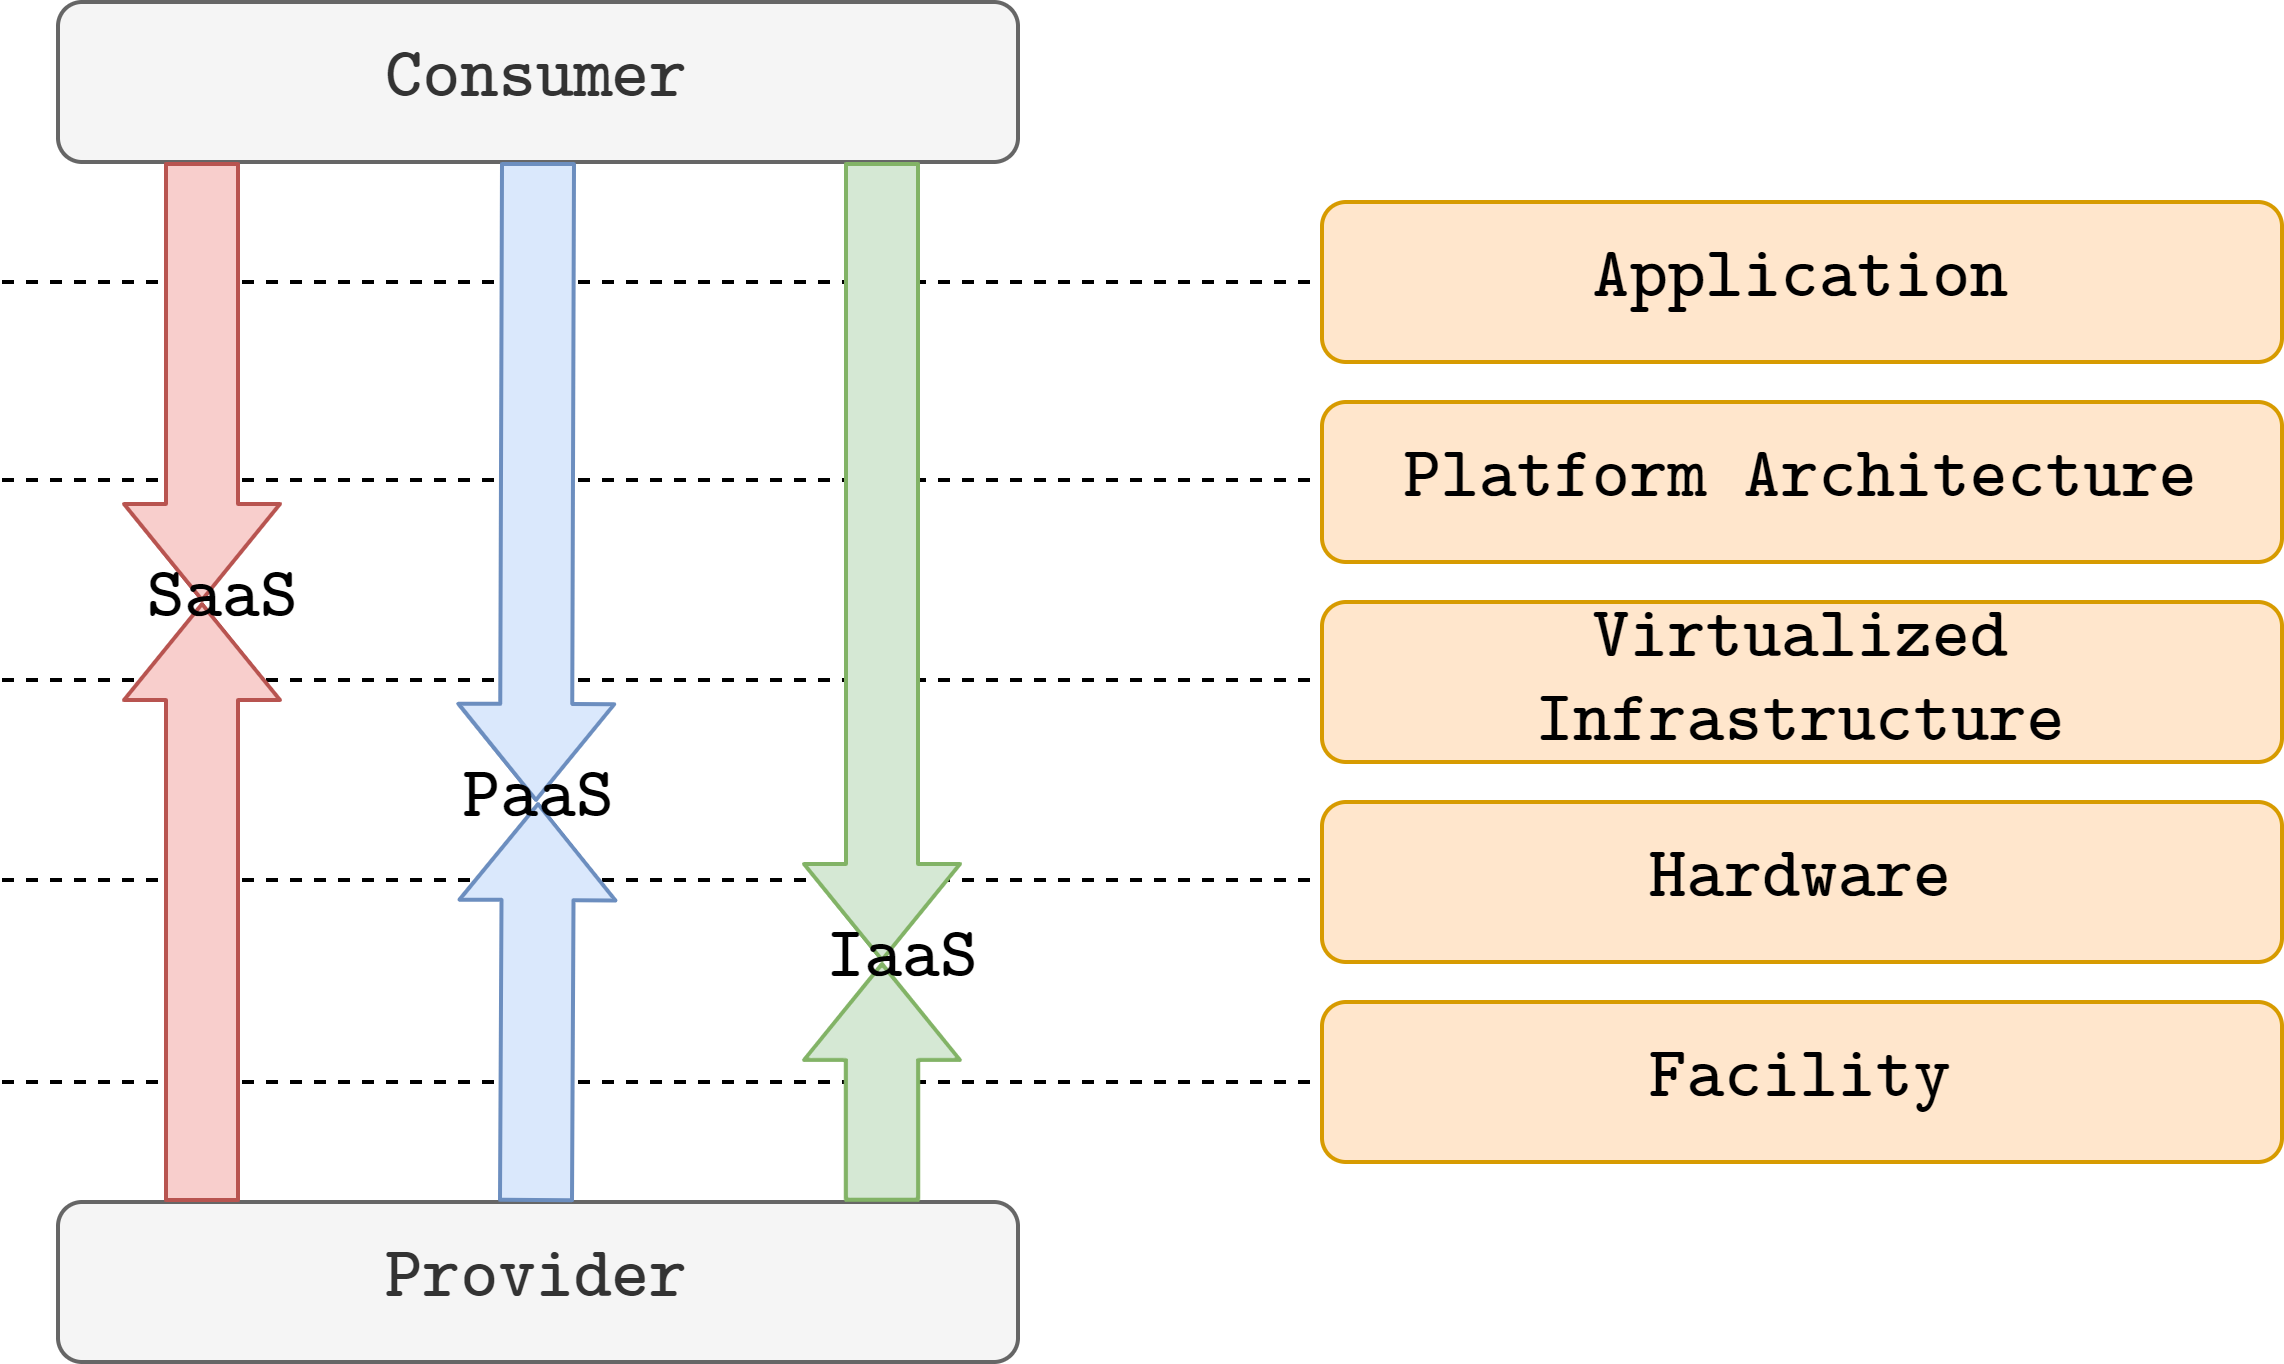
\includegraphics[width=8cm]{./Images/cap7/7.4.png}
\end{figure}

\section{Case Study: ATN}
ATN (nome fittizio) è un'azienda che fornisce network equipment a livello mondiale ed è cresciuta in maniera significativa attraverso diverse acquisizioni di aziende specializzate per componenti internet, gsm e cellulari. Adesso è un fornitore di punta di un'ampia gamma di infrastruttura di rete, cellulari e telecomunicazioni. 

A causa di queste acquisizioni il sistema è diventato eterogeneo e quindi soggetto a forti pressioni da parte del mercato. Il costo quindi aumenta per mantenere la gestione dei reparti IT con i partner in tutto il mondo. Sembra utile a questo punto adottare il cloud, viene quindi stabilita una roadmap producendo una serie di vantaggi tra cui abbreviare gli investimenti a breve termine e i costi a lungo termine, cercando di ottenere un'ottimizzazione del servizio e una riduzione di costi con i soliti vantaggi di scalabilità, availability e business. ATN deve capire quale modello adottare e quindi quale offre più vantaggi, contando però dei problemi: potrebbero infatti perdere il controllo sulle loro applicazioni, e inoltre va considerato il fatto che bisogna avere fiducia nel cloud provider per quanto riguarda le compliance. Un altro problema è rappresentato dalle legacy applications e come devono essere integrate.

\vspace{5mm}

Viene suggerito di provvedere ad una valutazione delle applicazioni sulla base di alcuni fattori quali complessità, business critical, frequenza di utilizzo e numero di utenti attivi, in modo da identificare i candidati per la migrazione sul cloud. Per ognuno dei candidati si fa un assessment usando un tool proprietario e poi si suggerisce lo sviluppo di un'architettura target che rende evidente l'interazione tra le applicazioni cloud based e l'infrastruttura esistente. Infine va fatto un piano di sviluppo.

Gli analisti ATN individuano una serie di rischi: tra le applicazioni delle varie aziende che sono state acquisite ce n'è una che ha il problema degli accessi differenti, non utilizza password complesse e la comunicazione tra i dati non è cifrata. Viene quindi deciso di non migrare quest'applicazione sul cloud, perché i rischi sono troppi e il rapporto prestazioni/prezzo non soddisfa gli obiettivi dell'azienda.

Quindi abbiamo visto come non sempre il cloud sia la soluzione giusta.

\section{Learning Check}
\begin{enumerate}
    \item Descrivi i principali threat agents relativi al cloud computing, tra cui: Anonymous Attacker, Malicious Service Agent, Trusted Attacker, Malicious Insider.
    \item Descrivi la minacca alla sicurezza del malicious intermediary, come può compromettere l'integrità e la confidenzialità dei messaggi e come questi attacchi possono essere portati a termine da servizi guidati da eventi.
    \item Descrivi la minaccia alla sicurezza Denial of Service e come viene eseguita sovraccaricando l'utilizzo della memoria e del processore.
    \item Descrivi la minaccia alla sicurezza delle autorizzazioni insufficienti e come una variante di questa minaccia è conosciuta come “weak authentication.”.
    \item Descrivi la minaccia alla sicurezza noto come virtualization attack, come mai è specifico delle risorse IT virtualizzate e come può essere portato avanti da un cloud service consumer fidato.
    \item Descrivi la minaccia degli overlapping trust boundaries e come risulta da diversi cloud consumer che condividono le stesse risorse IT cloud-based.
    \item Spiega ulteriormente le vulnerabilità associate ad implementazioni imperfette, disparità nelle policy di sicurezza e l'importanza del risk management.
    \item Descrivi il caso d'uso di ATN e le motivazioni delle decisioni prese.
\end{enumerate}
